\documentclass[modern, letterpaper]{aastex62}
% \documentclass[twocolumn, letterpaper]{aastex62}

% to-do list
% ----------
% - Review: http://adsabs.harvard.edu/abs/2008EAS....29....1M (sec 4.6)
% - https://ui.adsabs.harvard.edu/#abs/2016A%26A...593A.133B/abstract
% - What can we say about tidal theory, given that our stars have a range of ages?

\include{gitstuff}
% Load common packages
% \usepackage{microtype}  % ALWAYS!
\usepackage{amsmath}
\usepackage{amsfonts}
\usepackage{amssymb}
\usepackage{booktabs}

\usepackage{graphicx}
\usepackage{color}

\definecolor{cbblue}{HTML}{3182bd}
\usepackage{hyperref}
\definecolor{linkcolor}{rgb}{0.02,0.35,0.55}
\definecolor{citecolor}{rgb}{0.45,0.45,0.45}
\hypersetup{colorlinks=true,linkcolor=linkcolor,citecolor=citecolor,
            filecolor=linkcolor,urlcolor=linkcolor}
\hypersetup{pageanchor=true}

\newcommand{\documentname}{\textsl{Article}}
\newcommand{\sectionname}{Section}
\renewcommand{\figurename}{Figure}
\newcommand{\eqname}{Equation}
\renewcommand{\tablename}{Table}

% Packages / projects / programming
\newcommand{\package}[1]{\textsl{#1}}
\newcommand{\acronym}[1]{{\small{#1}}}
\newcommand{\github}{\package{GitHub}}
\newcommand{\python}{\package{Python}}
\newcommand{\emcee}{\project{emcee}}

% Missions
\newcommand{\project}[1]{\textsl{#1}}

% For referee
\newcommand{\changes}[1]{{\color{red} #1}}

% Stats / probability
\newcommand{\given}{\,|\,}
\newcommand{\norm}{\mathcal{N}}

% Maths
\newcommand{\dd}{\mathrm{d}}
\newcommand{\transpose}[1]{{#1}^{\mathsf{T}}}
\newcommand{\inverse}[1]{{#1}^{-1}}
\newcommand{\argmin}{\operatornamewithlimits{argmin}}
\newcommand{\mean}[1]{\left< #1 \right>}

% Unit shortcuts
\newcommand{\msun}{\ensuremath{\mathrm{M}_\odot}}
\newcommand{\kms}{\ensuremath{\mathrm{km}~\mathrm{s}^{-1}}}
\newcommand{\mps}{\ensuremath{\mathrm{m}~\mathrm{s}^{-1}}}
\newcommand{\pc}{\ensuremath{\mathrm{pc}}}
\newcommand{\kpc}{\ensuremath{\mathrm{kpc}}}
\newcommand{\kmskpc}{\ensuremath{\mathrm{km}~\mathrm{s}^{-1}~\mathrm{kpc}^{-1}}}

% Misc.
\newcommand{\bs}[1]{\boldsymbol{#1}}
\definecolor{mahogany}{RGB}{165,15,21}
\newcommand{\resp}[1]{{\color{mahogany}#1}}

% Astronomy
\newcommand{\DM}{{\rm DM}}
\newcommand{\feh}{\ensuremath{{[{\rm Fe}/{\rm H}]}}}
\newcommand{\df}{\acronym{DF}}

% TO DO
\newcommand{\todo}[1]{{\color{red} TODO: #1}}


% adjust AAS-TEX shit
% \setlength{\parindent}{1.1\baselineskip}

\graphicspath{{figures/}}

% define macros for text
\newcommand{\apogee}{\project{\acronym{APOGEE}}}
\newcommand{\sdssiv}{\project{\acronym{SDSS-IV}}}
\newcommand{\thejoker}{\project{The~Joker}}
\newcommand{\thecannon}{\project{The~Cannon}}
\newcommand{\DR}{\acronym{DR14}}
\newcommand{\DRtw}{\acronym{DR12}}
\newcommand{\RC}{\acronym{RC}}
\newcommand{\RGB}{\acronym{RGB}}
\newcommand{\quantile}[2]{\ensuremath{\textrm{Q}_{#1}}\left(#2\right)}
\newcommand{\pdf}{\textit{pdf}}
\newcommand{\logg}{\ensuremath{\log g}}
\newcommand{\Teff}{\ensuremath{T_{\textrm{eff}}}}
\newcommand{\med}[1]{\ensuremath{\textrm{med}\left(#1\right)}}

\newcommand{\nunimodal}{322}
\newcommand{\nclean}{234}

% for response to referee
% \renewcommand{\resp}[1]{#1}

\shortauthors{Price-Whelan et al.}

\begin{document}\sloppy\sloppypar\raggedbottom\frenchspacing % trust me

\title{Binary companions of evolved stars in \apogee\ \DR: \\
       Orbital circularization}

\author[0000-0003-0872-7098]{Adrian~M.~Price-Whelan}
\affiliation{Department of Astrophysical Sciences,
             Princeton University, Princeton, NJ 08544, USA}
\email{adrn@astro.princeton.edu}
\correspondingauthor{Adrian M. Price-Whelan}

% \author[0000-0003-2866-9403]{David~W.~Hogg}
% \affiliation{Max-Planck-Institut f\"ur Astronomie,
%              K\"onigstuhl 17, D-69117 Heidelberg, Germany}
% \affiliation{Center for Cosmology and Particle Physics,
%              Department of Physics,
%              New York University, 726 Broadway,
%              New York, NY 10003, USA}
% \affiliation{Center for Data Science,
%              New York University, 60 Fifth Ave,
%              New York, NY 10011, USA}
% \affiliation{Flatiron Institute,
%              Simons Foundation,
%              162 Fifth Avenue,
%              New York, NY 10010, USA}

% \author[0000-0003-4996-9069]{Hans-Walter~Rix}
% \affiliation{Max-Planck-Institut f\"ur Astronomie,
%              K\"onigstuhl 17, D-69117 Heidelberg, Germany}

\begin{abstract}\noindent % trust me
% Context
Short-period binary stars tend to have circular orbits.
Orbital circularization a strong function of convective layer size.
% Aims
A sample of binary star systems with giant star member
Study circulariation vs. surface size.
% Methods
% Results
Circularization timescale must be shorter than evolutionary timescale
\end{abstract}

\keywords{
  binaries:~spectroscopic,
  --
  binaries:~close,
  --
  stars:~evolution,
  --
  stars:~interiors
}

\section{Introduction} \label{sec:intro}

From studies of binary star systems in open clusters, it is clear that
short-period binaries tend to be more circular (have smaller eccentricities) as
compared to longer-period binaries of the same age (e.g.,
\citealt{Mathieu:2005}).
Within a given population of binaries, this manifests as an apparently steep
transition from a spread in eccentricities to mainly circularized orbits
that occurs around some characteristic period (see, e.g., \figurename~5 in
\citealt{Mathieu:2005}).
This critical value of the period depends on the age and evolutionary state of
the population.
Many studies have measured the ``circularization period,'' predominantly for
main-sequence binaries (e.g., \citealt{Meibom:2006, Kjurkchieva:2017}), and have
found that it tends to be between 5--20 days, depending on age (e.g.,
\citealt{Mathieu:1988}).
For giant stars, the circularization period appears to be longer, closer to
$\approx 100$ days (\citealt{Mayor:1984}).
These observed trends are likely a result of orbital circularization rather than
a manifestation of binary star formation: The circularization or transition
period appears to vary with the age of the population (\citealt{Meibom:2005}).

Theories that explain orbital circularization generally rely on tidal
dissipation to explain and predict the timescales of this phenomenon (see
\citealt{Mazeh:2007hp} for a review).
For stars with deep convective zones (and especially evolved stars), the
\emph{equilibrium tide theory} (\citealt{Zahn:1977, Zahn:1989}) has been shown
to reasonably reproduce the circularization periods of a small sample of
binaries with giant star members in open clusters (\citealt{Verbunt:1995}).
In this theory, the tidal bulge induced on the primary (evolved) star will lag
the orbital motion of the companion because of coupling of the tidal flow to
turbulent eddies driven by convection.
These eddies cause an effective viscosity in the convective region of the
primary star, and the magnitude of this viscosity affects the amount of lag,
which directly relates to the circularization timescale for a given binary
system (\citealt{Zahn:1989}; also summarized in \citealt{Goodman:1997}).

The circularization timescale is a strong function of the ratio of the binary
separation, $a$, to the radius of the primary star, $R_1$ (assuming the primary
has begun to evolve off the main sequence and the secondary remains a
main-sequence star), with a scaling
\begin{equation}
    t_\textrm{circ} \propto \left(\frac{a}{R_1}\right)^8 \quad .
\end{equation}
Therefore for a given binary, even small changes in the radius of the primary
results in large changes in the circularization timescale.
For binary stars with periods $P \gtrsim 10~\textrm{day}$, we therefore expect
orbital circularization to begin only as the primary begins to evolve.
Further, if the circularization timescale remains short compared to the
evolutionary timescale along the subgiant and giant branches, then the
circularization period of a sample of binary stars should correlate with the
radius or evolutionary state of the primary.

Using a sample of binary star systems with at least one evolved member, we show
that indeed the inferred circularization period is a function of the surface
gravity of the primary star.
Assuming that our sample contains a small range in primary stellar masses, this
implies that there is a clear correlation between circularization period and
evolved stellar radius or depth of the convective region.

In \sectionname~\ref{sec:data}, we describe the original data source and catalog
of binary star systems used in this work.
In \sectionname~\ref{sec:results}, we show how the circularization period changes in bins of primary-star surface gravity.
In \sectionname~\ref{sec:discussion}, we discuss \todo{...}

\section{Data} \label{sec:data}

To identify binaries, we use sources with repeat radial velocity measurements in
data release 14 (\DR) of the \apogee\ survey
(\citealt{Majewski:2017,Abolfathi:2017}), a component of the Sloan Digital Sky
Survey IV (\sdssiv; \citealt{Gunn:2006,Blanton:2017}).
A full description of our search methodology and binary star catalogs can be
found in companion work (\citealt{Price-Whelan:2018}).

Briefly, we use a custom-built Monte Carlo sampler (\package{The Joker};
\citealt{Price-Whelan:2017}) to generate posterior samples over binary orbital
parameters (period, eccentricity, etc.) for all stars with $\geq 3$ radial
velocity measurements in \apogee\ \DR\ that pass a series of quality cuts.
By making cuts on our posterior belief about the amplitude of radial velocity
variations, we identified $\sim$5,000 binary star systems with at least one
evolved star member.
However, the majority of these systems have too few radial velocity measurements
to uniquely determine the binary orbital parameters.

Here, we only consider \nunimodal\ binary systems for which the period and
eccentricity can be uniquely determined (the ``high-$K$, unimodal'' sample of
\citealt{Price-Whelan:2018}).
We further subselect the \nclean\ primary stars with $\logg > 2$ and that pass
visual inspection (from previous work, \texttt{clean\_flag == 0}; see
\sectionname~5.2 in \citealt{Price-Whelan:2018}).

\section{Expectations from theory and prior work}
\label{sec:theory}

Tidal circularization should happen fast for binary star systems with a giant
star member.
TODO: explain Verbunt and Phinney paper in more detail (\citealt{Verbunt:1995}; hereafter VP95)

Motivated by and following VP95, we generate a simulated population of binary
star systems with primary stars that have similar stellar parameters to our
sample of \apogee\ system primaries.
We assume simple initial binary orbital parameter distributions (i.e. in period
and eccentricity) and compute the change in eccentricity of the companion orbit
as the primary star evolves off the main sequence using equilibrium tide theory
(\citealt{Zahn:1966}, and see simplified expressions in VP95).

In detail, we generate primary stellar masses, companion masses, and primary
surface gravities by fitting two-component Gaussian mixture models (GMMs) to the
stars in our sample with measurements of each, then re-sample using the fitted
distributions.
As described in previous work (\citealt{Price-Whelan:2018}), primary mass
measurements come from \cite{Ness:2015}, (minimum) secondary masses come from
the posterior samplings over orbital parameters using \apogee\ radial velocity
data, and surface gravities come from the \apogee\ (\DR) data reduction pipeline
(\citealt{Garcia-Perez:2016}).
In our sample, the median primary mass, companion mass, and surface gravity are
$\med{M_1} = 1.4~\msun$, $\med{M_{2, \textrm{min}}} = 0.4~\msun$, and
$\med{\logg} = 3.1$.

To follow the stellar evolution of the primary, we run stellar evolution models
using \acronym{MESA} \citealt{Paxton:2011} for stars with $M = [1, 1.2, 1.4,
1.6, 1.8, 2, 2.5, 3]~\msun$, from the pre-main-sequence phase until $\logg = 0$
(i.e. near the tip of the giant branch); We assume solar metallicity for these
simulations.
At each timestep during the evolution, we output and store the standard stellar
parameters along with the size and mass of the convective envelope.

We discretize the primary masses generated from the GMMs onto the grid of masses
for which we have \acronym{MESA} models, then use equilibrium tide theory to
compute the change in eccentricity of the companion orbit.
To do this, we integrate \equationname~\ref{} up to the phase of evolution at
which the stellar model has the same (or closest) surface gravity to the
simulated primary star.
Here we assume that all stars are on their first ascent up the giant branch,
which should underestimate the number of circularized systems with surface
gravities $\logg \sim 2.5$ (i.e. near the red clump, where stars have already
reached the tip of the giant branch).
We also assume that the equilibrium tides dominate the circularization process
for all systems and therefore ignore the effect of ``dynamical tides''
(\citealt{who}) during the main sequence phase.
Finally, following VP95, we also assume that the semi-major axis of the binary
system stays constant as the eccentricity damps.

\figurename~\ref{fig:XX} shows the initial (left) and final (middle and right)
periods and eccentricities of the simulated systems.
In the right panel, we normalize the orbital period by the orbital period of a
hypothetical, massless companion whose pericentric distance grazes the surface
of the primary star,
\begin{align}
    P_{\textrm{surface}} &= 2\pi \, \left(\frac{M_1+M_2}{M_1}\right) \,
        \left(\frac{G\,M_1}{R_1^3}\right)^{-1/2} \, \left(1-e\right)^{-3/2}
    \quad .
\end{align}
Markers are colored by the log-surface gravity, \logg, and the size indicates
the mass of the primary.

\section{Results}
\label{sec:results}

\figurename~\ref{fig:XX} shows orbital period and eccentricity

The samples produced in this work provide excellent datasets to study tidal
circularization of companions to giant stars across a range of ages and
metallicities
However, our samples consist of a mix of subgiants, giants, and RC stars which
have distinct distributions in mass and stellar radius.
To visualize the distribution of systems in period--eccentricity space, we have
therefore computed normalized periods, where we normalize by the orbital period
of a typical companion on a circular orbit at the surface of the primary,
$P_{\textrm{surface}}$.
To do this for all systems in this sample, we assume that all primary stars have
masses equal to the median mass over all stars with prior mass measurements in
this sample, $M_1 = 1.36~\msun$, and assume a companion mass also equal to the
median over minimum companion masses $M_{2, \textrm{min}} = 0.5~\msun$.
We then use the surface gravity, $\log g$, of the primary, and eccentricity to
compute

where we use $M_{2, \textrm{min}}$ as $M_2$.

\figurename~\ref{fig:PeK}, left panel, shows this normalized orbital period and
eccentricity for all systems in the high-$K$, unimodal sample, and, right panel,
the RV semi-amplitude.
There is a clear signature of circularization just under $P/P_{\textrm{surface}}
\approx 10$.
\todo{what else can or should we say?}

% Notebook: Results
\begin{figure}[h]
\begin{center}
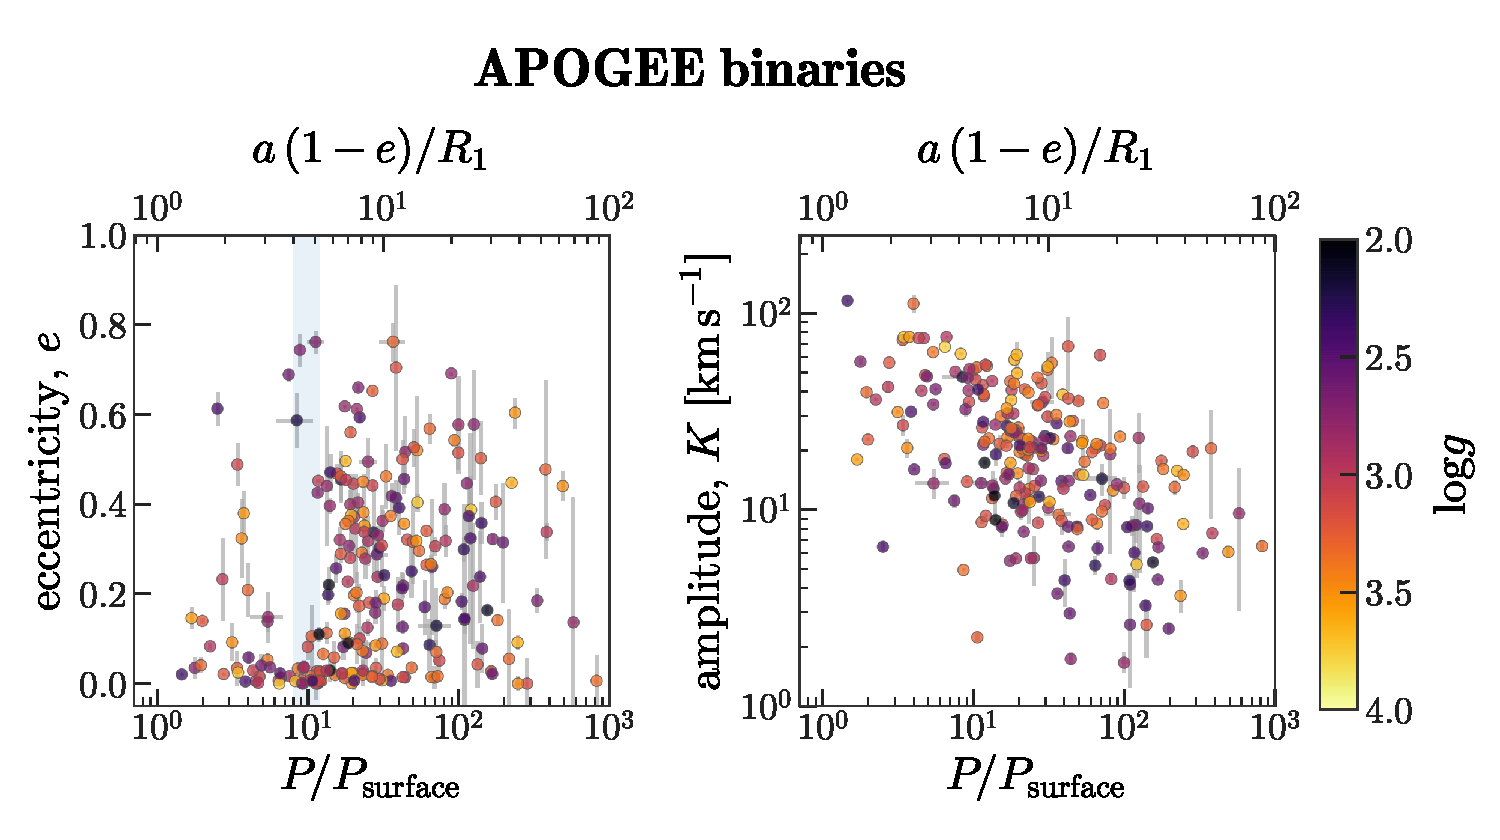
\includegraphics[width=\textwidth]{P-e-K}
\end{center}
\caption{%
\textit{Left panel:} Orbital period and eccentricity for all high-$K$ unimodal
systems with $\log g > 2$, with period values normalized by the orbital period
of a hypothetical companion at the surface of each primary star,
$P_{\textrm{surface}}$, assuming $M_1 = 1.36~\msun$ and $M_2 =0.5~\msun$.
Stars in the \apogee\ \DR\ red clump catalog are outlined in red.
The sharp transition from eccentric systems to almost all circular orbits at
$P/P_\textrm{surface} \approx 7$ is likely an outcome of tidal circularization.
\textit{Right panel:} Normalized period and inferred radial velocity amplitude
for the same systems.
Points below $P/P_\textrm{surface} = 1$ are likely systems where the primary and
companion mass assumptions used to compute $P_\textrm{surface}$ are invalid.
\label{fig:PeK}
}
\end{figure}


\section{Discussion} \label{sec:discussion}

- Low-ecc "spur" extends to larger periods. This could be: (a) systems where the companion already evolved (even more efficient), or (b) systems that started with smaller ecc. to begin with.


\section{Conclusions}



\acknowledgements

It is a pleasure to thank
Matteo Cantiello (Flatiron),
Jeremy Goodman (Princeton),
David W. Hogg (NYU/Flatiron/MPIA),
Hans-Walter Rix (MPIA),
and Joshua Winn (Princeton).

The authors are pleased to acknowledge that the work reported on in this
paper was substantially performed at the TIGRESS high performance computer
center at Princeton University which is jointly supported by the Princeton
Institute for Computational Science and Engineering and the Princeton
University Office of Information Technology's Research Computing department.

\software{
    \package{Astropy} (\citealt{Astropy-Collaboration:2013}),
    \package{emcee} (\citealt{Foreman-Mackey:2013}),
    \package{IPython} (\citealt{Perez:2007}),
    \package{matplotlib} (\citealt{Hunter:2007}),
    \package{numpy} (\citealt{Van-der-Walt:2011}),
    \package{scikit-learn} (\citealt{Pedregosa:2011}),
    \package{scipy} (\url{https://www.scipy.org/}),
    \package{schwimmbad} (\citealt{Price-Whelan:2017a}),
    \package{sqlalchemy} (\url{https://www.sqlalchemy.org/}),
    \package{thejoker} (\citealt{Price-Whelan:2017b}),
    \package{twobody} (\todo{twobody zenodo}).
}

\facility{\sdssiv, \apogee}

\clearpage

\bibliographystyle{aasjournal}
\bibliography{refs}


\end{document}
